%-------------------------------
\section{Produktdaten}
\label{sec:Produktdaten}
%-------------------------------

\subsection*{(Hannes Stadler)}

\begin{quote}
\begin{tabular}{p{1.5cm}p{14.5cm}}


	 /D10/	& \textbf{Datentyp:} Räume \\
				& \textbf{Attribute:} Raum ID \textsl{(systemintern)}, Raumnummer, Gebäude, Stockwerk, Sitzplätze, PC-Plätze, Beamer, Visualizer, Overheads, Tafeln, Whiteboards  \\[0.25cm]

\end{tabular}


\begin{tabular}{p{1.5cm}p{14.5cm}}
		
	 /D20/	& \textbf{Datentyp:} Lehrstühle \\
				& \textbf{Attribute:} Lehrstuhl ID \textsl{(systemintern)}, Lehrstuhlname, Lehrstuhlinhaber, Fakultät, Gebäude (für die zukünftige Erweiterung), (Haupt-)Stockwerk  \\[0.25cm]

\end{tabular}


\begin{tabular}{p{1.5cm}p{14.5cm}}
					
	 /D30/	& \textbf{Datentyp:} Benutzer \\
				& \textbf{Attribute:} Benutzer ID \textsl{(systemintern)}, Benutzerkennung, Passwort (Hash), Salt, E-Mail, Benutzerzugehörigkeit (Verwaltung, betreffender Lehrstuhl, wünschenswerterweise auch Student), Vorname, Nachname, letzter Login  \\[0.25cm]

\end{tabular}


\begin{tabular}{p{1.5cm}p{14.5cm}}
					
	 /D31/	& \textbf{Datentyp:} Dozenten \\
				& \textbf{Attribute:} Dozenten ID \textsl{(systemintern)}, Benutzer ID, Lehrstuhl ID  \\[0.25cm]

\end{tabular}


\begin{tabular}{p{1.5cm}p{14.5cm}}
	
	 /D50/	& \textbf{Datentyp:} Lehrveranstaltungen \\
				& \textbf{Attribute:} Veranstaltungs ID \textsl{(systemintern)}, Benutzer ID (Dozent), Veranstaltungskurzbezeichnung, Veranstaltungsname, Semester, Benötigte SWS, Art (Vorlesung|Übung|Tutorium), Freigabe durch Dozent, Beschreibung, Erwartete Teilnehmer\\ 
				&(Tag, Zeiteinheiten, etc. wird über "`Raumbelegung [siehe /D60/]"' ermittelt, wo für jede Zeiteinheit ein Eintrag erstellt wird und Veranstaltungen mehrere Einträge pro Semester buchen können.) \\[0.25cm]

\end{tabular}


\begin{tabular}{p{1.5cm}p{14.5cm}}
					
	 /D60/	& \textbf{Datentyp:} Raumbelegungen (aller Freigabestatus-Arten) \\
				& \textbf{Attribute:} Belegungs ID \textsl{(systemintern)}, Veranstaltungs ID (Lehrveranstaltung), Raum ID, Semester, Tag, Zeiteinheit, Freigabestatus (unbearbeite|freigegeben|abgelehtn|gegenvorschlag), Freigabenachricht (Falls ein Vorschlag abgelehnt wurde und dies nun ein reservierter Vorschlag des Status "`gegenvorschlag"' ist), Kommentar  \\[0.25cm]

\end{tabular}


\begin{tabular}{p{1.5cm}p{14.5cm}}
		
	 /DW70/& \textbf{Datentyp:} Studentensammlung \\
				& \textbf{Attribute:} Studenten-Sammlungs ID \textsl{(systemintern)}, Benutzer ID (Student), Belegungs ID (freigegebene Lehrveranstaltung) \\[0.25cm]

\end{tabular}


\begin{tabular}{p{1.5cm}p{14.5cm}}
					
	 /DW80/& \textbf{Datentyp:} Ticker-Nachricht \\
				& \textbf{Attribute:} Meldungs ID \textsl{(systemintern)}, Meldungstext, Start-Datum, End-Datum \\[0.25cm]
		
\end{tabular}

\begin{tabular}{p{1.5cm}p{14.5cm}}
					
	 /DW90/& \textbf{Datentyp:} Ticker-Zuordnung \\
				& \textbf{Attribute:} Ticker-Zuordnungs ID \textsl{(systemintern)}, Meldungs ID, Belegungs ID, Veranstaltungs ID, Lehrstuhl ID, Raum ID \\[0.25cm]
		
\end{tabular}


Im Structured-Entity-Relationship-Modell (SERM, siehe Abbild \ref{fig:dbserm}) wird der Zusammenhang der oben spezifizierten persistent zu speichernden Daten verdeutlicht. \\

\begin{figure}[H]
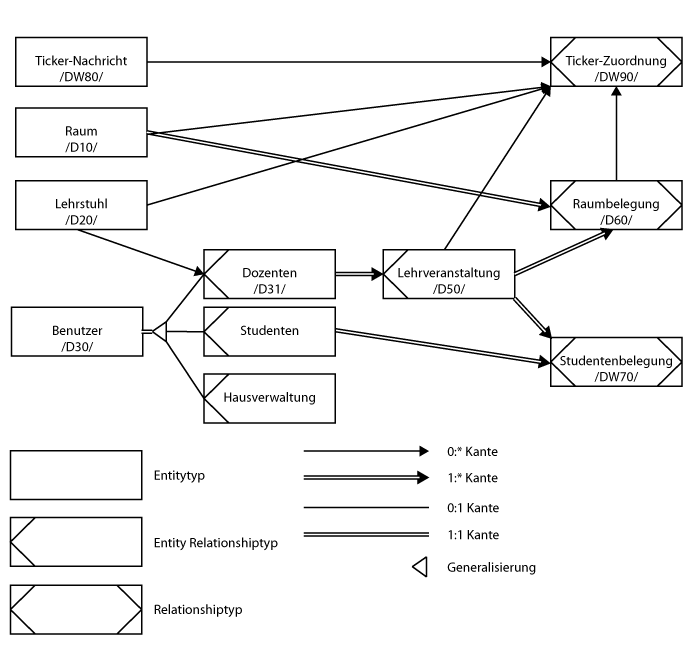
\includegraphics[scale=0.70]{./images/section_5/dbserm}
\caption{SERM der Daten-Architektur}
\label{fig:dbserm}
\end{figure}

Wie in der Abbildung zu sehen ist, existieren Räume, Lehrstühle, Benutzer und Ticker-Nachrichten als eigenständige Einheiten (Entity). Benutzer können einem Lehrstuhl zugeordnet werden, womit sie der Klasse "`Dozent"' entsprechen. Sie können aber auch der Klasse "`Verwaltung"' oder "`Student"' angehören und somit keiner anderen Einheit zugeordnet werden. Lehrveranstaltungen müssen einem Dozent zuzuordnen sein. Eine Raumbelegung ist keine Einheit sondern eine Zuordnung (Relationship) und muss einer Lehrveranstaltung und einem Raum zugeordnet werden können. Die Zuordnung Studentenbelegung muss einem Student und einer Lehrveranstaltung zugeordnet werden können. Ticker-Nachrichten können einem Raum, einer Lehrveranstaltung, einem Lehrstuhl, einer Raumbelegung oder allen Einheiten davon zugeordnet werden, nichts davon ist jedoch zwingend (existiert kein Zuordnungseintrag zu einer Ticker-Nachricht, so ist sie global gültig). \\


\end{quote}